\chapter{Investigation of Visualization Tools using a Feature Classification Scheme}
\label{chap:Tools}

In this section we analyze selected visualization tools and their ability to visualize large time-oriented data. Therefore, the database metrics were compared for each tool. Database metrics is one part of the definition of visual scalability and describe how tools scale to large data sets. A detailed discussion can be found at section \ref{databasemetrics}. Moreover, we developed a classification scheme which is based on the collected success criteria of chapter \ref{chap:BIV} and ranked the tools according to this classification scheme. \\*

\section{Selection of Tools}\label{tool:selection}
The tools were selected based on their relevance in business. Nowadays, businesses strive to do self-service data science\cite{Russom2011,Parenteau2016,visualization2012making,curran2005self}. Therefore, they use self-service tools which are characterized by a graphical user interface (GUI), low prior programming skills and the universal use. The GUI enables non computer scientists to analyze data by the help of the human visual system. According to ITCentralStation and the Magic Quadrant for Business Intelligence and Analytics Platforms 2017 \cite{ITCentralStation, Sallam2017} and  Qlik, Tableau and Microsoft are the leading visionaries of BI Vendors. All of these tools proclaim to support the user in data visualization, self-service data science and to be easy to use. Thus, Qlik, Tableau and Microsoft Power BI are popular visualization tools (\ref{tools}). Their strength lies in the user support and their universality. Nevertheless, each tool is fee-based which results in investment costs. \\
Commercial software tends to need more time for the development and integration of advanced visualization for large data\cite{Zhanga, Simon2014}. Therefore, we added an open-source visualization tool to our selection. d3.js is a well-known choice for visualization in the visualization community as it is a free open-source JavaScript library and offers a wide range of visualization possibilities. \\
Thus, the selection of tools are Qlik Sense, Tableau, Microsoft Power Bi and d3.js.

%Nevertheless, market relevance reports from research and advisory companies such as Gartner, Forrester, Barc usually do not publish detailed scoring models.  Thus, the ranking might not be appropriate to our needs.


% \iffalse
% ADV in business context requires software that is able to scale visualization in an "effective manner"\cite{Russom2011}. Offering ADV techniques, parameterization, interaction and analytical methods such as data abstraction\cite{Tegarden1999,Aigner2011,Eick2002,Zhanga} are core functions of ADV software. \\*
% \textbf{The Role of APIs}
% Commercial software tends to need more time for the development and integration of advanced visualization for large data\cite{Zhanga, Simon2014}. To bridge the gap, vendors started to offer a bunch of APIs to expand the visualization functions. 
% % data load for BigData: 
% \textbf{Software not included in this work}
% As the goal of this work is to compare visualization tools in business we only consider software which is 
% \begin{enumerate}
%     \item generic: not specialized to one domain
%     \item integrates visualization features
% \end{enumerate}

% Furthermore, the software needs visualization features, the ability to present time-dependent data. Software with one of the following items is intentionally not considered: 
% \begin{enumerate}
%     \item Software that only presents one-dimensional data. 
%     \item Software that is specialized to data mining.
% \end{enumerate}
% \fi

\textbf{Qlik Sense: }
Qlik Sense is the self-service product of Qliktech. Qliktech was founded in 1993 with the goal to "mimic how the brain works."\cite{qlikHistory}. They offer five products(QS, QS Cloud, QlikView, QlikView NPrinting, Qlik DataMarket) and the Qlik Analytics platform. QS 1.0 was released in September 2014 for visual analytics. 
Self-Service data visualization describes the approach to encourage a broad public to do data analysis with easy-to-use tools.\\
\textbf{Power BI: }
Microsoft Power BI came alive in September 2013. It is divided in the three services Power BI Mobile, Power BI Desktop and Power BI service. Power BI Mobile access reports by a portable device. Power BI Desktop is a business analytics suite for creating visualizations and reports and Power BI service publishes reports. We are concentrating on Power BI Desktop.\\
\textbf{Tableau: }
Tableau was founded in 2003 out of a university project. Tableau sells three main products: Tableau Desktop, Tableau Public and Tableau Server.\\ 
\textbf{d3.js: }
d3.js is a JavaScript library used for visualization. It visualizes data based on SVG, HTML5 and CSS and binds data to existing web elements in alignment with the Document Object Model (DOM).  Data Handling is managed by the underlying data source. Data modeling can be handled by other JavaScript libraries such as node.js. A good overview how d3.js works is given in \cite{Meeks}. 
We chose d3.js as it is a data visualization tool with interaction. As it is free it becomes an alternative to commercial tools.\\


\section{Scalability of visualization tools}\label{tool:scalability}
Visual scalability of visualization tools is measured by the \textit{database metrics} and the \textit{visualization characteristics}. Moreover, as discussed in \ref{chap:BIV} scalability is enhanced by analytical methods and interaction techniques. Thus, the scalability of visualization tools will be compared by determining database metrics, visualization characteristics, analytical and interaction abilities for each tool.

\subsection{Database metrics}
Database metrics are defined as the size of the database which can be handled by tools\cite{Eick2002}. One possibility to measure the database size are the number of lines which can be loaded into the tool. Another approach to measure database metrics are the maximum number of rows which can be loaded into a visualization.
\par
While \textbf{d3.js}, \textbf{Power BI} and \textbf{Tableau} have no limitations how many data rows can be loaded, \textbf{QS} inherits the data load limitations of Qlik View: A QS document cannot have more than 2,147,483,648 distinct values in one field. This limitation still allows Qlik to handle large and huge data sets according to our definition. Moreover, 2 billion data points exceed the limit of screen pixels. But nevertheless, QS is outperformed by d3.js, Power BI and Tableau in this particular case.
\par
In context of visualization the number of rows which are loaded into a visualization is a determining factor for scalability. For large data the user expects to load all data he wants the tool to load. However, some tools limit the initial number of rows and the user has to write additional code. This effects the easy-of-use negatively.
QS limits the initial fetch to 10.000 but gives the opportunity to fetch more data if needed. \textbf{d3.js}, \textbf{Power BI} and \textbf{Tableau} currently have no limit for rows in visualization.
Again QS stays behind d3.js, Power BI and Tableau.

% Ranking for Database Metrics
\begin{table}[H]

    \begin{tabular}{|l| l l l l l|}
        \hline
        \multicolumn{2}{|c}{}   & d3.js  & QS  & Power BI & Tableau\\\hline
        \multirow{2}*{Database Metrics}
        & Maximum \# of rows in tool                & 1 & 4 & 1 & 1\\
        & Maximum \# of rows in visualization       & 1 & 4 & 1 & 1\\
        \hline
        \multicolumn{2}{|c}{}   & \textbf{1}    & \textbf{4}  & \textbf{1} & \textbf{1}\\
        \hline
    \end{tabular}
    \caption{Tool Ranking for criterion \textit{Database Metrics}}
    \end{table}

\subsection*{More than database metrics}
With the current development in technology, data management shifted from importing csv-files or Excel Spreadsheets to working with technologies such as clouds or databases. Thus, the maximum number of rows is no appropriate measure for database metrics anymore. Instead of measuring the loading time of data rows the connectivity to large scale cluster is the decisive factor. Most of the visualization tools today provide data engines, an underlying software component, which manages the data. Thus, the tool performance depends on the following factors:
\begin{enumerate}
    \item The underlying engine
    \item The connectivity to Big Data Technologies
\end{enumerate}
Other limiting factors are connection to multiple data sources, the perceived performance by the user and hardware resources.  Out of these factors visualization tools can influence the underlying engine, the connection, incremental loading and the connectivity to Big Data technologies. As this work focuses on the frontend perspective of scalability to large data sets the connectivity to Big Data Technology goes beyond the scope of this work. Here, we are shortly discussing the tool's underlying engine to make clear how the definition of database metrics needs to be adjusted. 

\textbf{The underlying Engine: In-memory versus Live Connection}
The architecture of engines in visualization tools can have the two forms: in-memory and live connection.
In-memory techniques store their data inside the RAM while live connections work directly on the database. 
With large data sets in-memory technologies might not be feasible. Even though working in-memory is faster than working directly at the database. With a smaller subset of large databases working in-memory might be the better option. 
\textbf{QS} data engine (QIX Engine) and \textbf{Power BI} use in-memory columnbased technology. While the data engine processes the calculation the RAM may temporarily be allocated. Thus, QS is limited by the primary memory of the computer. \textbf{Power BI} extends also to live connections to clouds similar to \textbf{Tableau}. Both tools offer in-memory technology as well as live connection. Tableau promotes the use of live connections instead of working in-memory even though working in-memory might be faster for small sets. Therefore, Tableau offers data extracts which can be created to work in-memory. The limits for data extracts are not published but Tableau Public, the free version of Tableau, recently extended the limit of 1 mio. rows to 10 mio. rows in-memory. 
d3.js is build to manage the visual frontend for visualizations. The data loading is outsourced to the backend. Therefore, d3.js can connect with any backend which implements the REST API. Thus, d3.js can not be compared with QS, Power BI and Tableau in this context. 
In summery, QS only offers in-memory and thus, has difficulties to work live on large data sets. Tableau and Power BI outperform QS in the criterion of database metrics.\\*
\textbf{Further Aspects: }
Scalability of tools can also be measured in terms of users and delivery. But this goes beyond our scope.


\subsection{Visualization Characteristics}

\subsubsection{The classification scheme}\label{tool:classification}\\*
The tools basis of assessment concerning \textit{visualization characteristics} is a classification scheme based on the success criteria of section \ref{success}. These aspects are assessed according to two business relevant criteria for self-service tools: the criterion of completeness and the criterion of required programming skills. The factor \textit{completeness} serves as indicator how many features can the business user achieve with this tool. Completeness in aggregation metaphors displays how many visualization techniques include aggregation metaphors. Yet, completeness is difficult to measure. Thus, we compare completeness by relative comparison.
\begin{table}[H]
	\caption[Tool Completeness]{Criteria Completeness: extend to which assessed aspect is implemented in tool}
	\label{programming-skills}
	\begin{tabu}{cl}
	\hline
	Points & Criteria\\
	\hline
	0 & Not existing\\
	1 & partially implemented \\
	2 & fully implemented \\
	\hline
	\end{tabu}
\end{table}

The consideration of programming skills in business is important as the standard business user of the visualization tool may have few programming knowledge (compare \ref{tasks}). Moreover, programming skills are connected with investment costs. The higher the required programming skills the higher are the investment costs. Programming skills are measured by the required user knowledge to achieve a feature. Least effort is needed when the tool offers the feature automatically (4). The next step is to embed a feature via drag and drop (3). This step still does not require any programming skill. On the next level programming knowledge is required but in a popular programming language (2). A popular programming language such as R, Java, JavaScript, python, C can used in other environments as well which increases the probability that the user knows the language. The difference from Step 2 to Step 3 is much larger than the difference from Step 3 to Step 4. Thus, the ranking is not linear but ordinal. The most complex level is when a feature can only be implemented by a tool-specific programming language (1). Here, we assume that a tool-specific language requires additional training effort. 
\begin{table}[H]
	\centering
	\caption[Programming-Skills for Tools ]{Criteria Required Programming-Skills to use the assessed aspect}
	\label{programming-skills}
	\begin{tabu}{cl}
	\toprule
	Points & Criteria\\
	\midrule
	1 & Feature can be programmed, but in a tool-specific programming language\\
	2 & Feature can be programmed in a popular programming language (R,JavaScript,Java)\\
	3 & Available by drag and drop \\
	4 & Automatic support by tool\\
	\bottomrule
	\end{tabu}
\end{table}

The criteria completeness and programming skills have been combined in the tool criteria score (TCS). Each feature of the tool has been assigned a tuple consisting of (Programming Skills, Completeness). If the assessed aspect did not exist 0 was assigned.
Based on the assessment of different features  we draw our conclusion (\ref{conclusion}).


% \iffalse
% \subsection*{R}
% \textbf{Analytical Techniques}\\
% Out of the five tools R has the most extensive offer of analytical methods for time-series data. It is possible to detect patterns such as outliers with tsoutliers\cite{Chen1993} and clusters with tsclust\cite{Manso2015}, do advanced analytics with tswge\cite{tswge} and forecasting with zra\cite{zra}.
% \textbf{Visualization Techniques}\\
% R supports standard visualization such as histograms, line charts and scatter plots. Advanced visualization techniques for large data sets 
% \textbf{Aggregation}\\*
% In the maps-package R offers the possibility to adjust the resolution with the parameter resolution. Resolution 0 maps the whole database whereas a higher resolution collapes data points within the resolution to one single point. This option allows to aggregate data and to only show the perceptual important points (PIP).
% The bigvis and the hexbin package implement binning to condense large data sets\cite{Wickham2013}.
% \textbf{Pixel-oriented} Time Series are visualized with mvtsplot\cite{mvtsplot}. This package allows to compare multivariate time-series data.
% \textbf{Interaction Techniques}\\
% Plot\_ly()\cite{plotly} supports a brushing function with drill-down.
% Shiny supports panning and zooming as well as linking and brushing.
% Linked views are supported by plot\_ly() with and without shiny. 
% Fish-eye views are implemented in the fisheyeR() package. 
% The time range can be decreased by limiting the data range inside the code.
% Animation can be achieved by using plot\_ly() and ggploty(). Moreover, plot\_ly() offers linked animated views.
% \textit{Dygraphs} includes also navigational sliders called Range Selector, panning and zooming and brushing of data items.
% \fi

\subsubsection{Detailed Tool Description}\label{tool:tools}
Before the TCS is assigned each tool is analyzed in detail with regard to the success criteria. \\

\noindent \textbf{Qlik Sense}
\par
\textbf{Analytical Techniques}\\
QS integrates methods to reduce data. Often, the tool specific \href{https://help.qlik.com/en-US/sense/3.2/Subsystems/Hub/Content/ChartFunctions/SetAnalysis/set-analysis-expressions.htm}{set expressions (SE)} are required therefore. 
Horizontal data reduction is implemented in \href{https://help.qlik.com/en-US/sense/3.2/Content/Videos/Videos-dimensions-limitations.htm}{\textit{Dimension Limitations}}. The user can decide upon the number of columns which are displayed. 
Dimensions are aggregated with \href{https://help.qlik.com/en-US/sense/3.2/Subsystems/Hub/Content/Dimensions/calculated-dimensions.htm}{\textit{calculated dimensions}}. Therefore, one or more dimensions are combined and saved as a new dimension.
Data reduction is part of QS Server. With \href{https://help.qlik.com/en-US/sense/2.1/Subsystems/Hub/Content/Scripting/Security/dynamic-data-reduction.htm}{\textit{dynamic data reduction (DDR)}} rows can be hidden for a group of users. Data rows can be reduced using SQL inside the backend. Thus, data size is decreased. Internally, .QVD files compress data. 
At the frontend, the user can apply \href{https://help.qlik.com/en-US/sense/2.1/Subsystems/Hub/Content/Visualizations/FilterPane/filter-pane.htm}{\textit{filters}}. QS \href{https://help.qlik.com/en-US/sense/2.1/Content/Videos/Videos-assoc-selection-model.htm}{\textit{standard selection mode}} includes brushing \& linking so that the selections of one visualization are automatically copied to all other visualizations. Additionally, the user can drag and drop custom filters inside the dashboard. 
Data clustering in QS is implemented by \href{https://help.qlik.com/en-US/sense/3.2/Subsystems/Hub/Content/Scripting/AggregationFunctions/aggregation-functions.htm}{\textit{aggregation-functions}}. These use SE and range from basic (min,avg,max) to advanced statistical functions(linear regression, correlation). With these aggregation functions QS offers some analytical methods. Yet, QS has no integration to an analytical program.
\par

\textbf{Visualization Techniques}\\
QS offers \href{https://help.qlik.com/en-US/sense/2.1/Subsystems/Hub/Content/Visualizations/visualizations.htm}{8 built-in visualization techniques}: bar charts, line charts, pie charts, scatter plots, treemap, maps, combi charts and gauge charts. If an additional technique is wanted the user can either install one of the community's self-made extensions or he can build his own \href{https://help.qlik.com/en-US/sense-developer/3.2/Subsystems/Extensions/Content/extensions-getting-started.htm}{\textit{visualization extension}} with \textit{JavaScript} and \textit{QEXT} files\cite{qlikWorkbench}. QS provides an extension template which supports the user in writing its extensions. Moreover, Qlik provides 20 high-level-APIs which supports the user in writing a custom extension. However, the user needs to know JavaScript, html\cite{qlikVisExtensions}, as well as QS own QEXT-language. \\*
Out of the QS standard repertoire non of the visualization technique corresponds to the studied visualization techniques of chapter \ref{chap:BIV}. With d3.js it would be possible to build these visualization techniques and integrate them in QS. 
The embedding of JavaScript also allows \textbf{aggregation} in terms of multi-resolution and the use of aggregation markers. However, these advanced metaphors have to be implemented for each technique and thus are only available for some techniques. Moreover, the implementation requires coding-skills. 

In the field of built-in-aggregation markers QS offers data aggregation for one chart type: the scatter plot. Hereby, large data is aggregated by aggregation markers. When the scatter plot is shown at an overview level accumulated data points are represented by squares. Data density is mapped to the color attribute.  The darker the square the denser the data\cite{qlikScatter}. The so called \href{https://help.qlik.com/en-US/sense/2.1/Subsystems/Hub/Content/Visualizations/scatter plot/scatter-plot.htm}{\textit{Smart Data compression}(SDC)} is one implementation for the aggregation of large data amounts. However, SDC is only available for one technique and that is why QS still stays behind the present day requirements.


\begin{figure}[H]
    \centering
    \subfloat[QS]{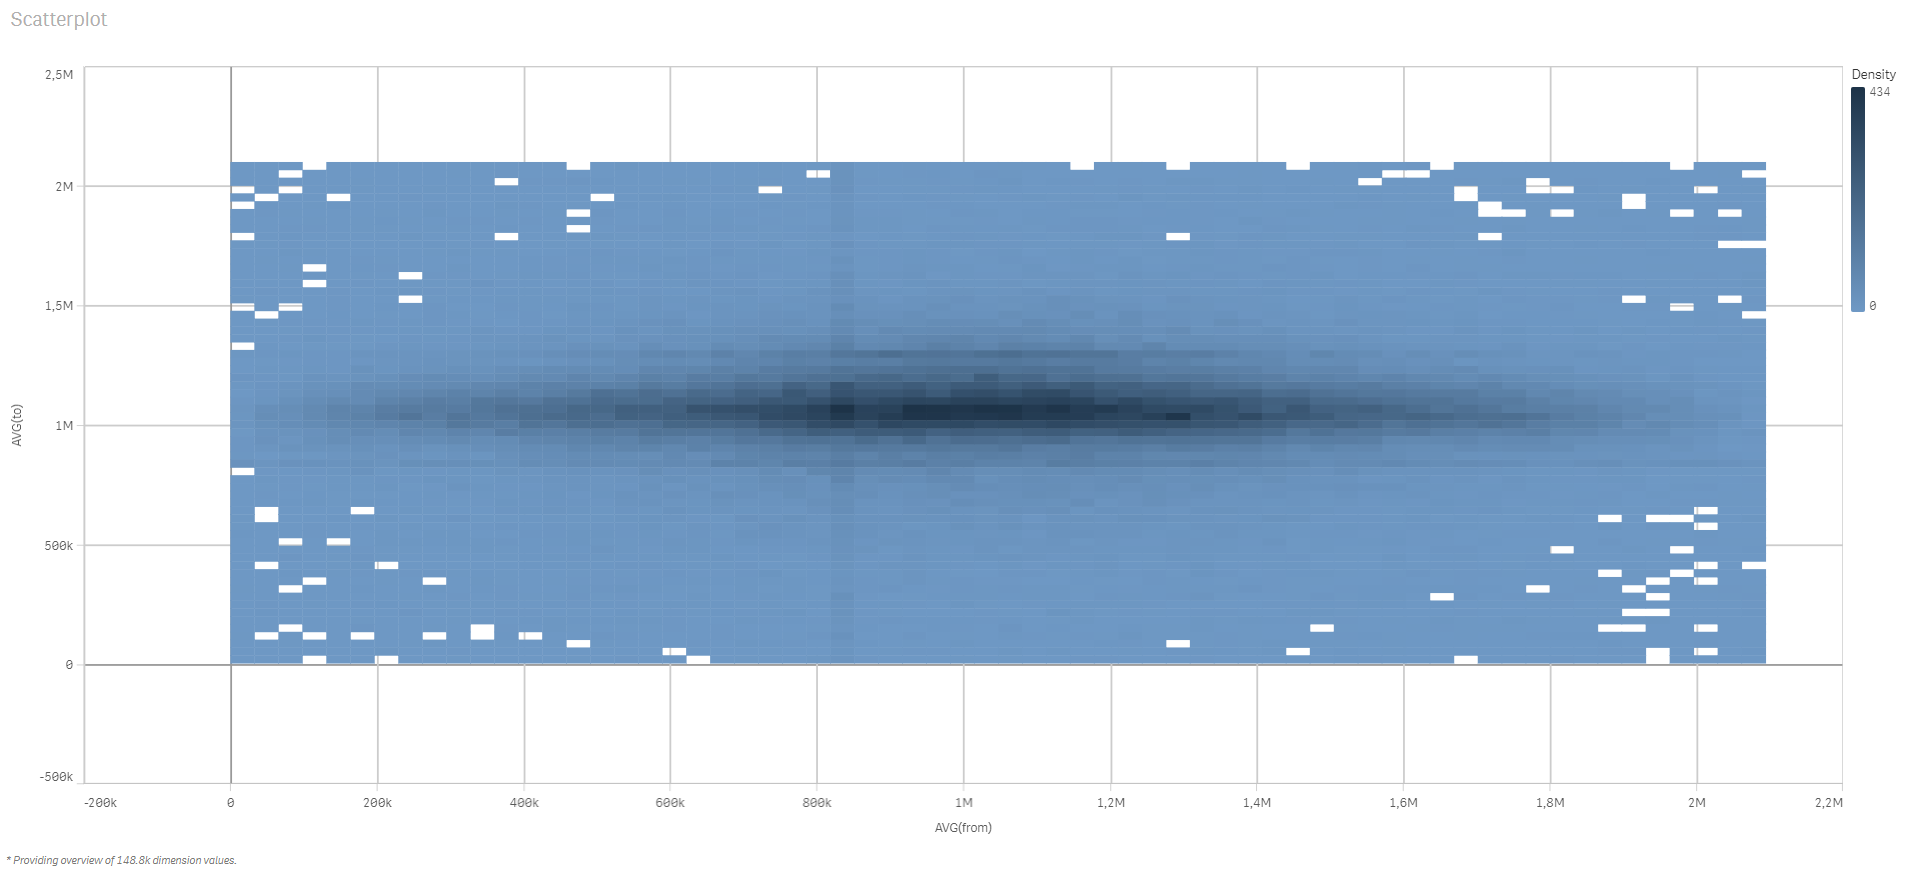
\includegraphics[width=6cm]{src/images/SmartDataCompression}}
    \caption{Smart Data Compression (left): Overview level which shows aggregated data points by squares and color and changes the shape if zoomed in}
    \label{fig:smartdatacompression}
\end{figure}

\begin{figure}[H]
    \centering
    \subfloat[Sparse Area]{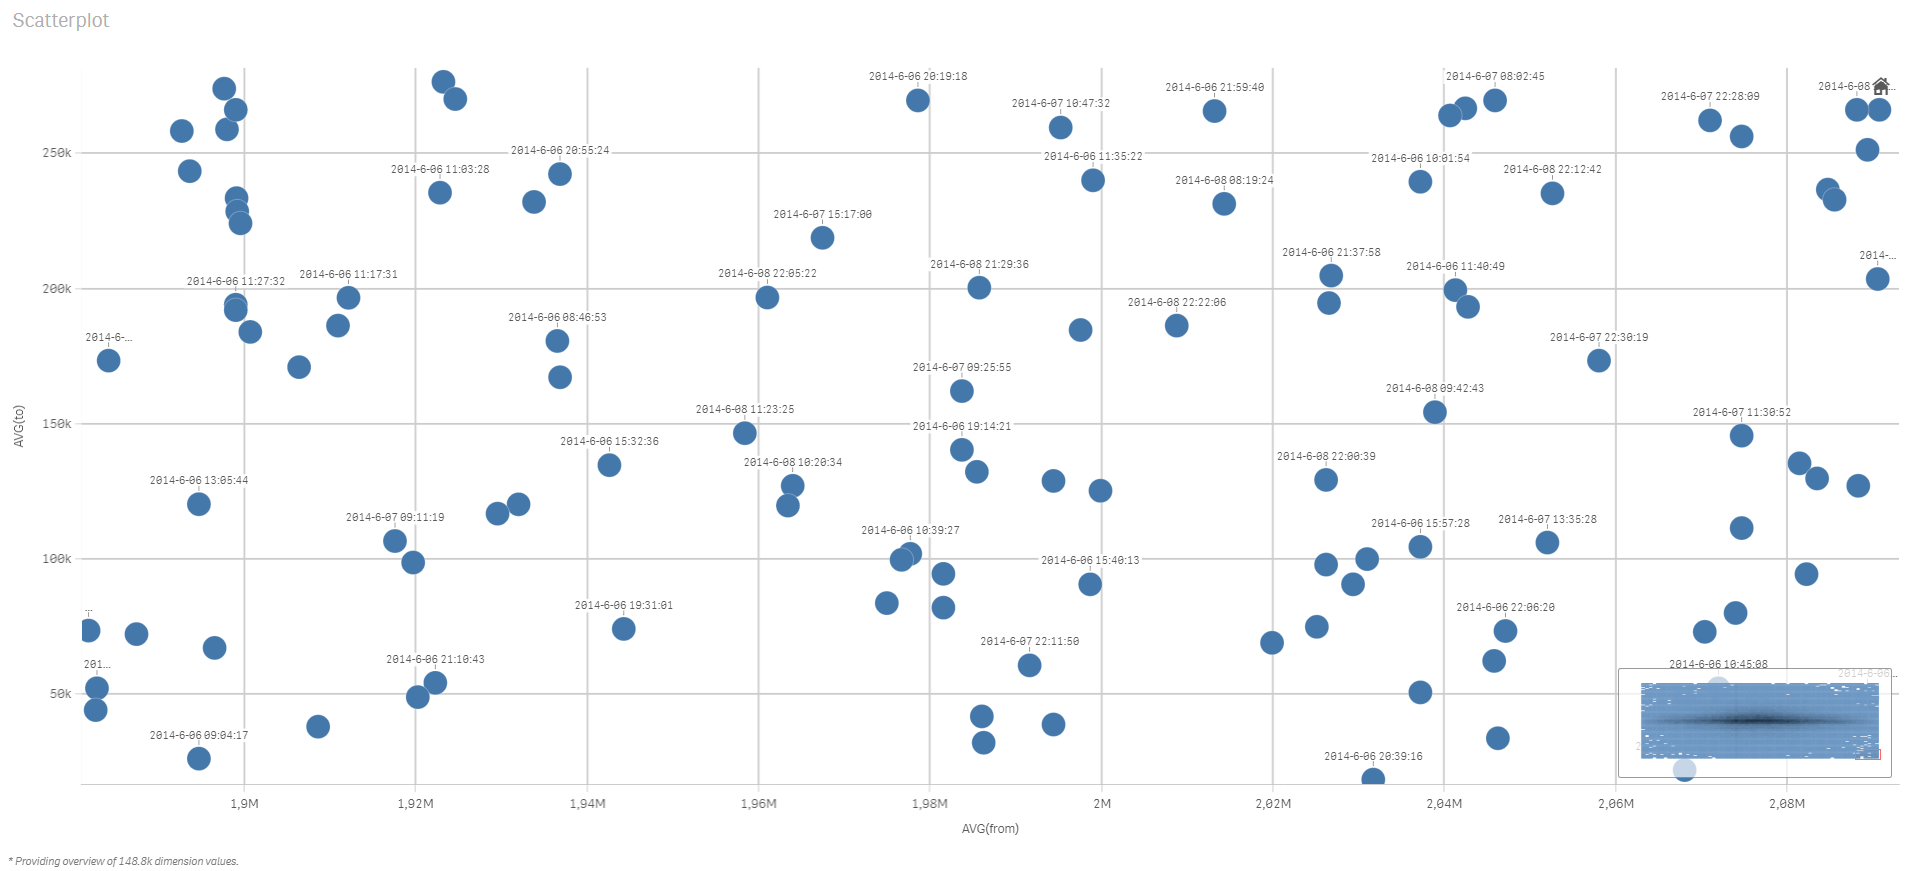
\includegraphics[width=6cm]{src/images/SmartDataCompressionI}}
    \qquad
    \subfloat[Dense Area]{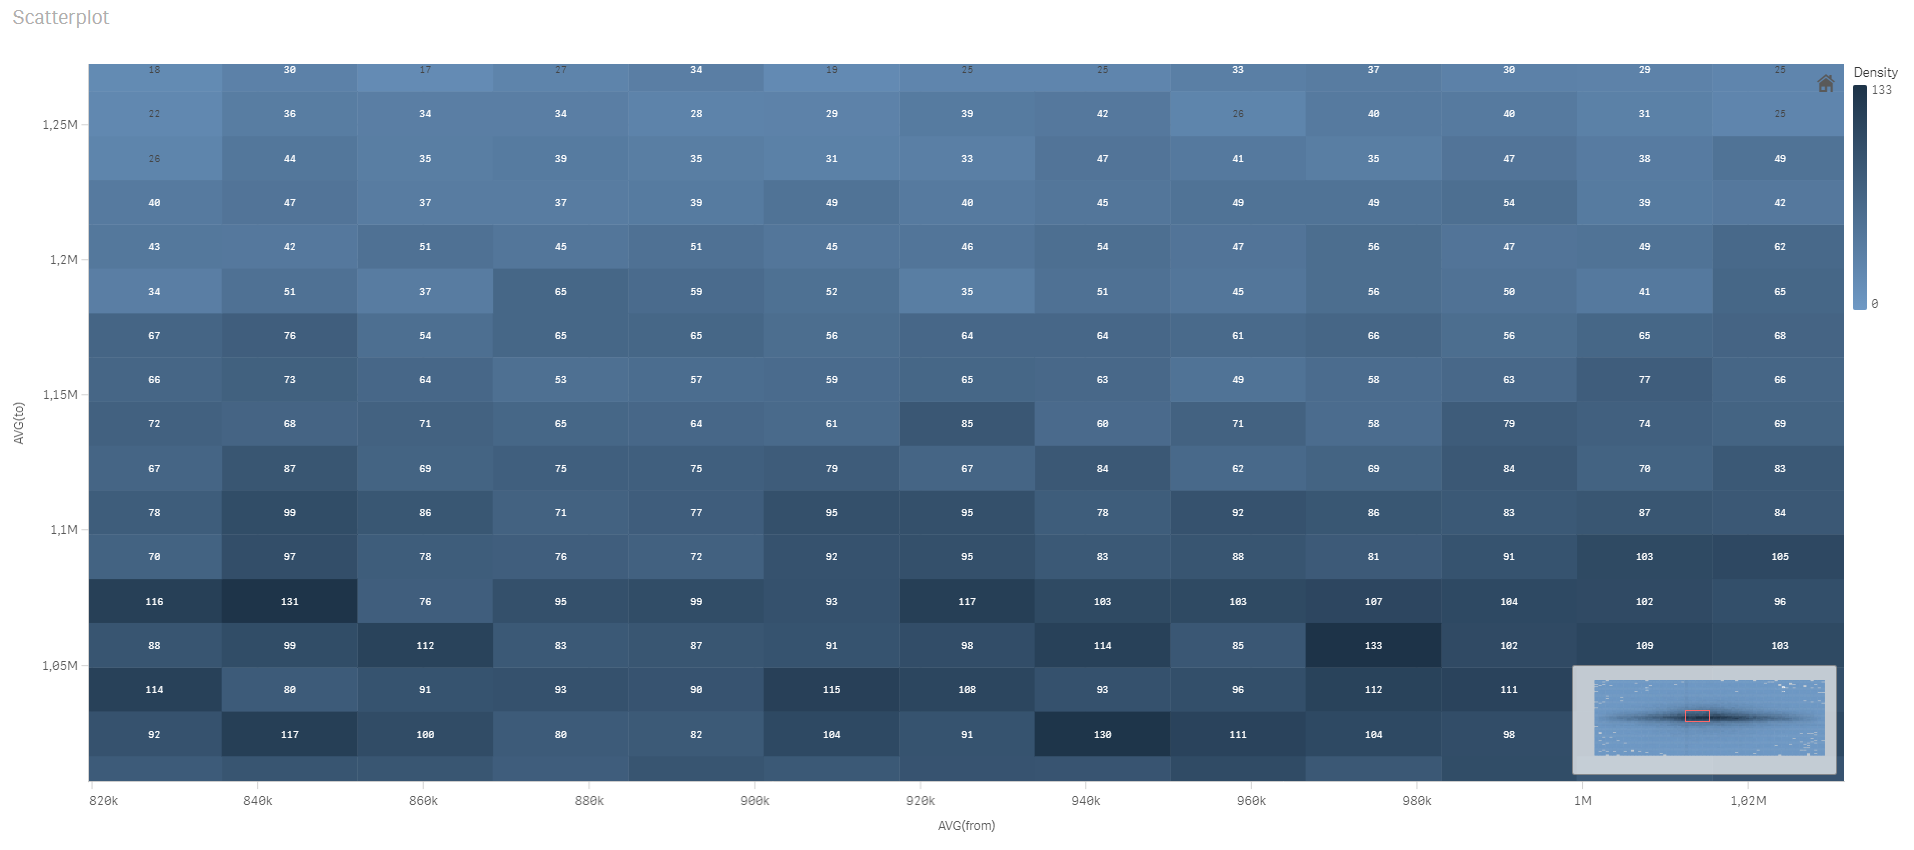
\includegraphics[width=6cm]{src/images/SmartDataCompressionII}}
    \caption{Smart Data Compression: Detail level}
    \label{fig:smartdatacompression}
\end{figure}

\textbf{Interaction Techniques}\\
In terms of interaction techniques QS offers drill-down and navigation techniques. Zooming and filtering are possible for all visualizations. If the zoom is active mini charts (MiC) appear which are one implementation of navigational maps\cite{beard1990navigational}. Mini Charts come as a navigational slider in which a miniature version of the whole data set\cite{beard1990navigational} is shown. 
Filters can be applied by making selections or dragging a filter inside the visualization\cite{qlikSheet}. All views then are adapted to the current selection. Thus, QS offers Brushing + Linking. For details the user can search QS with \href{https://help.qlik.com/en-US/sense/2.1/Content/Videos/Videos-global-smart-search.htm}{\textit{Smart Search}} in which the dimensions, measures and metadata is searched and visualizations, tables and KPIs are displayed\cite{qlikSmart}. Distortion techniques are not offered but can be implemented with extensions. 
\par
\noindent \textbf{Tableau}
\par
\textbf{Analytical Techniques}\\
Tableau's strength are easy-to-use analytical functions. On one hand, Tableau offers build-in modelling functions: prediction, trend line, cluster, average and median. On the other hand data reduction are offered and R scripts can be loaded into Tableau. Horizontal and vertical reduction is implemented by \href{http://onlinehelp.tableau.com/current/pro/desktop/en-us/extracting_data.html}{\textit{Data Extracts (DE)}}. These can be build based on the loaded data connection and remove reduce the data by limiting the loaded data. Dimensions can be reduced by hiding columns while creating DE. Only visible columns are then loaded into the dashboard. Dimensions are aggregated similar to QS by \href{http://onlinehelp.tableau.com/current/pro/desktop/en-us/calculations_calculatedfields.html}{\textit{calculated fields}}. Moreover,  \href{http://onlinehelp.tableau.com/current/pro/desktop/en-us/calculations_calculatedfields_aggregate.html}{\textit{aggregated calculations}} reduce data vertically by clustering them. Another implementation of vertical data reduction are  \href{http://kb.tableau.com/articles/howto/adding-filters-to-dashboards}{\textit{filter}} which can be added in the frontend. Tableaus analytical capabilities can be enhanced by integrating R which offers additional data reduction capabilities such as PCA or SOM.
\par
\textbf{Visualization Techniques}\\
Tableau offers 22 built-in visualization techniques: heat maps, symbol maps, stacked bars, pie charts, horizontal bars, side-by-side bars, treemaps, circle views, side-by-side circles, continuous lines, discrete lines, dual lines, area charts,  discrete area charts, dual combination, scatter plots, histogram, box-and-whisker plots, Gantt chart, bullet graphs and packed bubbles.
Visualization extensions are not possible even though Tableau has a \href{https://www.google.de/search?client=safari&rls=en&q=tableau+javascript+api&ie=UTF-8&oe=UTF-8&gfe_rd=cr&ei=2oLOWKveK5LZ8AeXl4bIBw}{JavaScript API}. This API allows the integration of a Tableau dashboard into a web page, but is not built for writing JavaScript extensions for Tableau. Besides, advanced metahpors such as multi-resolution, data abstraction or aggregation markers are not supported. 
In sum, Tableau is a well-known choice in the visualization community. But it does not support large scale visualization features. 
\par

\textbf{Interaction Techniques}\\
Speaking of drill-down techniques Tableau offers automatically zooming and  \hyperlink{http://kb.tableau.com/articles/howto/adding-filters-to-dashboards}{filtering}.
Regarding navigation techniques Tableau integrates \href{https://www.tableau.com/de-de/whitepapers/enhancing-visual-analysis-linking-multiple-views-data}{\textit{multiple linked views}}.
Distortion techniques, search and navigational sliders are not supported. 
\par

\noindent \textbf{Power BI}
\par
\textbf{Analytical Techniques}\\
Data reduction in Power BI is implemented similar to QS and Tableau. Dimensions can be aggregated with 
Horizontal data reduction implemented by  \href{https://powerbi.microsoft.com/en-us/documentation/powerbi-desktop-tutorial-create-calculated-columns/}{\textit{calculated columns}}. Vertically, data can be reduced both in the frontend and in the frontend. With \href{https://community.powerbi.com/t5/Desktop/How-to-reduce-the-amount-of-data-that-is-loaded-into-my-Power-BI/td-p/54112}{\textit{views}} on the database (V) and joins data extracts are created. Moreover, data sets can be extracted (DE) in the frontend with \href{https://Power BI.microsoft.com/de-de/blog/power-bi-desktop-october-feature-summary/#grouping}{\textit{Inclusion/Exclusion}} of data points. Moreover, \href{https://powerbi.microsoft.com/en-us/documentation/powerbi-service-add-a-filter-to-a-report/}{\textit{filters}} can be added and  \href{https://powerbi.microsoft.com/en-us/documentation/powerbi-service-aggregates/}{\textit{aggregates}} build.
Besides the own core functions for data reduction Power BI is connected to analytical programs such as \href{https://Power BI.microsoft.com/de-de/blog/power-bi-desktop-october-feature-summary/#grouping}{\textit{R, Mixpanel or comScore.}}
\par

\textbf{Visualization Techniques}\\
Microsoft Power BI offers 8 built-in \href{https://powerbi.microsoft.com/en-us/documentation/powerbi-service-visualization-types-for-reports-and-q-and-a/}{\textit{visualization techniques}}, 15 available techniques at the MarketPlace and 75 visualization apps in the visuals gallery. Additionally, the user can build custom visualization apps by writing \href{https://powerbi.microsoft.com/en-us/documentation/powerbi-custom-visuals-getting-started-with-developer-tools/}{\textit{TypeScript}} or \href{https://powerbi.microsoft.com/en-us/guided-learning/powerbi-learning-3-11h-r-visual-integration/}{\textit{R}}. Out of the 98 techniques none of them implements any discussed techniques of chapter \ref{chap:BIV}. So far advanced Metaphors are not supported\cite{Amanda}. One approach to aggregation markers are \hyperlink{https://Power BI.microsoft.com/de-de/blog/power-bi-desktop-october-feature-summary/#grouping}{\textit{Groups}} which can be combined with drill-down options.
\par

\textbf{Interaction Techniques}\\
Power BI embeds zoom and filter functions. The \textit{focus mode} expands one visualization to full screen and thus, enables the user to have a detailed view on the visualization. Thus, Power BI implements an overview + detail view. 
With \href{https://powerbi.microsoft.com/en-us/documentation/powerbi-service-about-filters-and-highlighting-in-reports/}{\textit{highlighting}} Power BI includes brushing and linking\cite{Power BIInteract}. Therefore, the user can control which windows are connected. The app \textit{Advanced Time Slicer} is one implementation of the navigation technique navigational map for time-oriented data. Navigation in Power BI is also realized by the search mechanism Power Q\&A which answers NLP-question regarding the data set. Power Q&A includes filtering with the keywords WHERE, AFTER, BEFORE, BETWEEN, WITH or by naming the date as well. Distortion techniques are not supported. They can be embedded with visualization extensions (E) written in TypeScript.

\par
\noindent \textbf{d3.js}
\par
\textbf{Analytical Techniques}\\
While d3.js is only designed to visualize data it does not inherently offer the ability to analyze data. Therefore, a number of JavaScript libraries (L) exist which can be combined with d3.js. Some examples are simplestatistics.js, regression.js, node.js with the packages data-reduction, ml-pca or dimensionality-reduction. As JavaScript allows the integration of libraries there is no limit for analytical functions. Thus, d3.js does not offer any data reduction techniques automatically. Besides libraries d3.js can be used together with any REST API compatible backend and the data reduction abilities then depend on the backend.
Regarding data abstraction d3.js offers abstraction functions the frontend. Some examples are d3.hexbin which allows binning, simplify.js for data abstraction or clusterfck for clustering. Simplify.js for example reduces data points on polylines while maintaining the characteristic shape of the polyline. 
\par

\textbf{Visualization Techniques}\\
d3.js assigns data attributes to graphical attributes. Thus, different way exist to visualize the same visualization technique. By writing JavaScript code any visualization technique and any advanced metaphor can be implemented. Currently, various implementations are \href{https://github.com/d3/d3/wiki/Gallery}{\textit{available}} which helps the user to create its own visualizations. For aggregation metaphors \href{http://bl.ocks.org/gisminister/10001728}{\textit{marker clustering}} is one example. Moreover, tutorials exist which describe how marker clustering can be implemented with  \href{https://www.phase2technology.com/blog/using-d3-quadtrees-to-power-an-interactive-map-for-bonnier-corporation/}{quadtrees}\cite{Morrison2014}.
\par

\textbf{Interaction Techniques}\\
d3.js allows to integrate various interaction techniques such as Zooming, Filtering or Linking \& Brushing. Distortion techniques can be achieved with the d3 plugin \hyperlink{https://bost.ocks.org/mike/fisheye/}{\textit{Fisheye Distortion (FD)}}\cite{Bostock2012} which allows circular, linear and logarithmic distortion.
Perspective walls can be implemented with \hyperlink{https://bl.ocks.org/mbostock/10571478}{\textit{Perspective Transformation (PT) }}\cite{Bostock2017}.\\

\subsubsection{Ranking of Tools}
All tool-features are listed in table \ref{table:features} and in table \ref{table:TCS} the TCS is derived. Then, the tools are ranked from the first place (1) to the last place(4). The first place is characterized by offering most of the features for large scale visualization relative to the other tools. Nevertheless, the first place is no optimum. 

\begin{table}[H]

    \begin{tabular}{|l| l l l l l|}
        \hline
        \multicolumn{2}{|c}{}   & d3.js  & QS  & Power BI & Tableau\\\hline
        \multirow{9}*{Analytics}
        & \multicolumn{5}{l|}{\cellcolor{gray!30} Horizontal Data Reduction}\\\cline{2-6}
        & Data can be reduced to $k$ dimensions & L & DL & - & H \\
        & Dimensions can be aggregated & L & CD & CC & CF\\ \cline{2-6}
        & \multicolumn{5}{l|}{\cellcolor{gray!30}Vertical Data Reduction}\\\cline{2-6} 
        & Omitting & L & DDR & J,V & DE,E\\
        & Filtering & L & DQ,B & DQ & DE,DQ,B\\
        & Removal & L & O & DE & DE \\
        & Abstraction & L & - & - & - \\
        & Aggregation & L & A & A & A \\\cline{2-6}
        &\rowcolor{gray!30}  Data Modeling & L  & -    & T,MM    & T, MM, F \\\cline{2-6}
        &\rowcolor{gray!30}  Pattern Search& L  & -    & -       & - \\
        \hline
        \multirow{3}*{Visualization}
        & Offers ADV                & P     & E    & E &-   \\
        & Multi-Resolution          & P     & E    & E & -  \\
        & Aggregation Markers       & MC    & SDC  & E & -  \\
        
        \hline
        \multirow{11}*{Interaction}
        
        & \multicolumn{5}{l|}{\cellcolor{gray!30}Drill-Down Functions}\\\cline{2-6}
        & Filter    & P & N & N & N \\
        & Zoom      & P & N & N & N \\ \cline{2-6}
        
        & \multicolumn{5}{l|}{\cellcolor{gray!30}Distortion Techniques}\\\cline{2-6}
        & Graphical Fish-eye    & \hyperlink{https://bost.ocks.org/mike/fisheye/}{FD}\cite{Bostock2012}       & E  & E  & - \\
        & Bifocal-Display       & \hyperlink{https://bost.ocks.org/mike/fisheye/}{FD}\cite{Bostock2012}       & E  & E  & - \\
        & Perspective Walls     & PT & E & E & - \\ \cline{2-6}
        
        & \multicolumn{5}{l|}{\cellcolor{gray!30}Navigation Techniques}\\\cline{2-6}
        & Brushing \& Linking   & P & N & N & N \\
        & Search                &  L & \hyperlink{https://help.qlik.com/en-US/sense/2.2/Subsystems/Hub/Content/Search/search-tool.htm}{SS}& \hyperlink{https://powerbi.microsoft.com/en-us/documentation/powerbi-service-q-and-a/}{Q\&A}& - \\
        & Navigational Maps     & P & \hyperlink{https://help.qlik.com/en-US/sense/1.1/Subsystems/Hub/Content/Visualizations/BarChart/BarChart.htm}{MiC}  & -           & -\\
        \hline
    \end{tabular}
    \caption{Tool implementations of success criteria}
    \label{table:features}
    \end{table}
    
    Analytics\\*
    L = Library, B = Brushing, CC = Calculated Columns, CD = Calculated Dimensions, CF = Calculated Fields, DA = Data Abstraction, DL = Data Limitations, DDR = Dynamic Data Reduction, DE = Data Extraction, DQ = Dynamic Query Filtering, E = Extensions, F = Forecasting, H = Hide Columns in Data Extract, J = Joins, MM = Min-Max-Function, O = Omit row in SQL-Script, T = Trendline, V = Views, - = not existing
    \par 
    Visualization\\*
    P = Programmable, E = Extensions, MC = Marker Clustering, SDC = Smart Data Compression, - = not existing
    \par
    Interaction\\*
    E = Extensions, FD = Fisheye Distortion, MiC = Mini Charts, N = Natively Integrated, P = Programmable, PT = Perspective Tranformation, Q\&A = Question \& Answer,  SS = Smart Search, - = not existing

\begin{table}[H]

    \begin{tabular}{|l| l l l l l|}
        \hline
        \multicolumn{2}{|c}{}   & d3.js  & QS  & Power BI & Tableau\\\hline
        \multirow{9}*{Analytics}
        & \multicolumn{5}{l|}{\cellcolor{gray!30} Horizontal Data Reduction}\\\cline{2-6}
        & Data can be reduced to $k$ dimensions & 2,2 & 4,1 & 2,2 & 4,2 \\  
        & Dimensions can be aggregated & 2,2 & 1,2 & 1,2 & 4,2  \\\cline{2-6}
        & \multicolumn{5}{l|}{\cellcolor{gray!30}Vertical Data Reduction}\\\cline{2-6}
        & Omitting               & 2,2 & 2,2 & 2,2 & 4,2 \\
        & Filter    & 2,2 & 3,2/4,2 & 3,2 & 3,2/4,2\\
        & Removal   & 2,2 & 2,2 & 4,2 & 4,2 \\
        & Abstraction           & 2,2 & 0 & 0 & 0\\
        & Aggregation           & 2,2 & 1,2 & 3,1 & 3,2 \\\cline{2-6}
        &\rowcolor{gray!30} Data Modeling  & 2,2 & 1,1 & 3,1 & 3,1 \\\cline{2-6}
        &\rowcolor{gray!30} Pattern Search & 2,2 & 0 &  0  & 0\\
        \hline
        \multirow{3}*{Visualization}
        & Offers ADV            &   2,2  &  1,2 & 1,2 & 0  \\
        & Aggregation Markers   &   2,2  &  1,1/4,1 & 1,1 &  0 \\
        & Multi-Resolution      &   2,2  &  1,1 & 1,1 & 0  \\
        
        \hline
        \multirow{11}*{Interaction}
        
        & \rowcolor{gray!30}Drill-Down Functions & & & &\\\cline{2-6}
        & Filter  & 2,2 & 4,2 & 4,2 & 4,2 \\ 
        & Zoom    & 2,2 & 4,2 & 4,2 & 4,2 \\\cline{2-6}
        
        & \rowcolor{gray!30}Distortion Techniques & & & &\\\cline{2-6}
        & Graphical Fish-eye    & 2,2 & 1,1 & 1,1 & 0 \\
        & Bifocal-Display       & 2,2 & 1,1 & 1,1 & 0 \\
        & Perspective Walls     & 2,2 & 1,1 & 1,1 & 0 \\ \cline{2-6}
        
        & \rowcolor{gray!30}Navigation Techniques & & & &\\\cline{2-6}
        & Brushing \& Linking   & 2,2 & 4,2 & 4,2 & 4,2\\
        & Search                & 2,2 & 4,2 & 1,1 & 0 \\
        & Navigational Maps     & 2,2 & 4,2 & 2,1 & 0 \\
        \hline
    \end{tabular}
    \caption{TCS for tools}
    \label{table:TCS}
    \end{table}

% Ranking for Programming Skills
\begin{table}[H]

    \begin{tabular}{|l| l l l l l|}
        \hline
        \multicolumn{2}{|c}{}   & d3.js  & QS  & Power BI & Tableau\\\hline
        \multirow{5}*{Analytics}
        & \rowcolor{gray!30}            & \textbf{4} & \textbf{3} & \textbf{2} & \textbf{1}\\\cline{2-6}
        & Horizontal Data Reduction     & 3 & 2 & 4 & 1\\
        & Vertical Data Reduction       & 4 & 3 & 2 & 1\\
        & Data Modeling                 & 3 & 4 & 1 & 1\\
        & Pattern Search                & 1 & 4 & 4 & 4\\
        \hline
        \multirow{3}*{Visualization}
        & \rowcolor{gray!30}    & \textbf{2}    & \textbf{1} & \textbf{3} & -\\\cline{2-6}
        & Offers ADV            & 1 & 2 & 2 & 4 \\
        & Aggregation Markers   & 2 & 1 & 3 & 4 \\
        & Multi-Resolution      & 1 & 2 & 2 & 4  \\
        
        \hline
        \multirow{3}*{Interaction}
         & \rowcolor{gray!30}   & \textbf{3}    & \textbf{1} & \textbf{2} & \textbf{4}\\\cline{2-6}
        & Drill-Down Functions  & 4 & 1 & 1 & 1    \\
        & Distortion Techniques & 1 & 2 & 2 & -    \\        
        & Navigation Techniques & 3 & 1 & 2 & 4    \\
        \hline
        \hline
        \multicolumn{2}{|c}{}   & \textbf{4}    & \textbf{2}  & \textbf{3} & \textbf{1}\\
        \hline
    \end{tabular}
    \caption{Tool Ranking for criteria \textit{Programming Skills}}
    \end{table}

% Ranking for Completeness
\begin{table}[H]

    \begin{tabular}{|l| l l l l l|}
        \hline
        \multicolumn{2}{|c}{}   & d3.js  & QS  & Power BI & Tableau\\\hline
        \multirow{5}*{Analytics}
        & \rowcolor{gray!30}            & \textbf{1} & \textbf{3} & \textbf{4} & \textbf{2}\\\cline{2-6}
        & Horizontal Data Reduction     & 1 & 4 & 1 & 1\\
        & Vertical Data Reduction       & 1 & 2 & 4 & 2\\
        & Data Modeling                 & 1 & 4 & 4 & 4\\
        & Pattern Search                & 1 & 4 & 4 & 4\\
        \hline
        \multirow{3}*{Visualization}
        & \rowcolor{gray!30}            & \textbf{1} & \textbf{2} & \textbf{3} & \textbf{4}\\\cline{2-6}
        & Offers ADV            & 1 & 2 & 2 & 4 \\
        & Aggregation Markers   & 1 & 2 & 3 & 4 \\
        & Multi-Resolution      & 1 & 2 & 2 & 4  \\
        
        \hline
        \multirow{3}*{Interaction}
         & \rowcolor{gray!30}   & \textbf{1} & \textbf{2} & \textbf{3} & \textbf{4}\\\cline{2-6}
        & Drill-Down Functions  & 1 & 1 & 1 & 1    \\
        & Distortion Techniques & 1 & 2 & 2 & 4    \\        
        & Navigation Techniques & 1 & 1 & 3 & 4    \\
        \hline
        \hline
        \multicolumn{2}{|c}{}   & \textbf{1}  & \textbf{2}  & \textbf{3} & \textbf{4}\\
        \hline
    \end{tabular}
    \caption{Tool Ranking for criteria \textit{Completeness}}
    \end{table}

\newpage
\section{Conclusion}

The tool comparison demonstrates that there exists different strategies for visualizing  large data in visualization tools: the analytical strategy and the visualization/interaction strategy. Tableau's strength is the analytical data visualization with a focus of \textit{data preprocessing} which is shown in the \textit{ease-of-use} ranking. Tableau takes the first place and the second in the \textit{completeness} ranking as this tool offers a broad range of analytical functions automatically or the user can drag functions such as clustering and prediction inside the dashboard. Moreover, the integration of R exploits \textit{data reduction} techniques and time-oriented user tasks. Tableau  promotes the reduction of a data set before loading it into Tableau as some features are only available for reduced data extracts. These features are count distinct, offline access and incremental refresh. d3.js itself does not offer any analytical methods. But as d3.js is a JavaScript library it can be extended by other libraries which support data reduction, data modeling or pattern search. While comparing QS, Power BI, Tableau and d3.js one has to consider that JavaScript is a turing complete programming language. Thus, all success features defined in \ref{chap:BIV} can be programmed with JavaScript which explains the first rank of d3.js among all categories. Nevertheless, visualizing in d3.js requires programming-skills and time and thus, d3.js never took the first place in the \textit{programming-skills} ranking.
On the contrary QS' lacks in analytical options. While Tableau can integrate R-algorithms to reduce data, QS only can manipulate data with the QS specific set expressions. However, set expressions are limited in data reduction possibilities.\\
Power BI combines both analytical and visualization features. One can build visualizations with R and TypeScript, and also execute R scripts in Power BI. \\
Still, the support of analytic techniques for time-oriented user tasks is only partially implemented. Tableau and Power BI provide forecasting but analytical techniques for time-oriented such as temporal abstraction or pattern search are not provided by any tool at the moment.
\par

The Visualization strategy goes along with interaction as both consider the frontend for visualizations. QS pursues that strategy which is shown in first implementations of aggregation markers with Smart Data Compression and the extendability. Its strength is the JavaScript-interface in which new visualizations can be integrated into QS. \\
Similar to QS visualization extensions are supported by Power BI whereas Tableau's support of visualization techniques lacks of ADV visualizations. Besides the standard repertoire no extensions can be installed. Hence, visualization of many data items currently lead to clutter and disorientation. As d3.js is a JavaScript library any visualization and advanced visual metaphor can be created.
The tool comparison regarding visualization showed that ADV requires the use of programming languages. Current visualization tools offer a standard repertoire of visualizations. These techniques are easy to use as they apply drag and drop. Yet, none of the techniques for multivariate time-oriented data is implemented by Tableau, QS or Power BI. Therefore, extensions are required which are implemented in a programming language. Furthermore, the languages for visualization extensions include tool specific languages such as Type Script and QEXT.\\
\par
Large-scale interaction techniques show the following pattern. Either they are automatically integrated in tools such as drill-down functions or they are not implemented in any tool such as distortion functions. The only way to integrate distortion functions are via extensions. Then the particular interaction technique is only available for the respective visualization technique. Yet, interaction techniques should general be available for every visualization technique.
Regarding navigation techniques coordinated windows are supported by all tools while QS and Power BI are the only tool which implements search. QS then is the only tool which provides navigational maps.
In short, all tools lack in distortion techniques and Tableau and Power BI in navigation techniques. 
\par
In summary, currently there exists no all-in-one solution for the analysis of large time-oriented data in business. While d3.js any possibility regarding visualization and  interaction programming knowledge is required. However, this conflicts with the business approach to do self-service data science. When business decide to use tools such as Tableau, QS and Power BI they need to be aware about the limitations in displaying large data in an effective manner. 



